\documentclass[12pt,fleqn]{article}\usepackage{../../common}
\begin{document}
Ay'a Gidelim, Kisitlanmis 3-Cisim Problemi (Restricted 3-Body Problem)

two body, space dyn - 374, 524, 553

szebehely pg 418

analyti-schaub 509

\begin{minted}[fontsize=\footnotesize]{python}
import numpy as np
import scipy
from scipy.integrate import odeint
from mpl_toolkits.mplot3d import Axes3D
from scipy.optimize import brentq
from scipy.optimize import fsolve
import pylab

mu1 = 398600;
mu2 = 4903.02;
mu = mu1 + mu2;
m1 = 5974e21;
pi1 = m1/M;
me = 5.974 * 10 ** 24  #  dunya kutlesi
mm = 7.348 * 10 ** 22  #  ay kulesi
G = 6.67259 * 10 ** -20  #  yercekimsel parametre
re = 6378.0  #  dunya yaricapi
rm = 1737.0  #  ay yaricapi
r12 = 384400.0  #  dunya mermezi ile ay merkez arasi mesafe
M = me + mm
d = 200  #  uzay tasitinin dunya uzerinden olan uzakligi
pi2 = mm / M
mue = 398600.0  #  gravitational parameter of earth km^3/sec^2
mum = G * mm  #  grav param of the moon
omega = np.sqrt(mu / r12 ** 3)
vbo = 10.9148
nu = -np.pi*0.5
gamma = 20*np.pi/180.0  #  angle in radians of the flight path

vx = vbo * (np.sin(gamma) * np.cos(nu) - np.cos(gamma) * np.sin(nu))
#  velocity of the bo in the x direction
vy = vbo * (np.sin(gamma) * np.sin(nu) + np.cos(gamma) * np.cos(nu))
#  velocity of the bo in the y direction

xrel = (re + d)*np.cos(nu)-pi2*r12
#  spacecraft x location relative to the earth
yrel = (re + 200.0) * np.sin(nu)

u0 = [xrel, yrel, 0, vx, vy, 0]

def deriv(u, dt):
    return [u[3],  #  dotu[0] = u[3]
            u[4],  #  dotu[1] = u[4]
            u[5],  #  dotu[2] = u[5]
            (2 * omega * u[4] + omega ** 2 * u[0] - mue * (u[0] + pi2 * r12) /
             np.sqrt(((u[0] + pi2 * r12) ** 2 + u[1] ** 2) ** 3) - mum *
             (u[0] - pi1 * r12) /
             np.sqrt(((u[0] - pi1 * r12) ** 2 + u[1] ** 2) ** 3)),
            #  dotu[3] = that
            (-2 * omega * u[3] + omega ** 2 * u[1] - mue * u[1] /
             np.sqrt(((u[0] + pi2 * r12) ** 2 + u[1] ** 2) ** 3) - mum * u[1] /
             np.sqrt(((u[0] - pi1 * r12) ** 2 + u[1] ** 2) ** 3)),
            #  dotu[4] = that
            0]  #  dotu[5] = 0


dt = np.linspace(0.0, 535000.0, 535000.0)  #  secs to run the simulation
u = odeint(deriv, u0, dt)

x, y, z, x2, y2, z2 = u.T

# 3d plot
fig = pylab.figure()
ax = fig.add_subplot(111, projection='3d')
ax.plot(x, y, z, color = 'r')

# 2d plot if you want
#fig2 = pylab.figure(2)
#ax2 = fig2.add_subplot(111)
#ax2.plot(x, y, color = 'r')

#  adding the moon
phi = np.linspace(0, 2 * np.pi, 100)
theta = np.linspace(0, np.pi, 100)
xm = rm * np.outer(np.cos(phi), np.sin(theta)) + r12 - pi2 * r12
ym = rm * np.outer(np.sin(phi), np.sin(theta))
zm = rm * np.outer(np.ones(np.size(phi)), np.cos(theta))
ax.plot_surface(xm, ym, zm, color = '#696969', linewidth = 0)
ax.auto_scale_xyz([-8000, 385000], [-8000, 385000], [-8000, 385000])
#  adding the earth
xe = re * np.outer(np.cos(phi), np.sin(theta)) - pi2 * r12
ye = re * np.outer(np.sin(phi), np.sin(theta))
ze = re * np.outer(np.ones(np.size(phi)), np.cos(theta))
ax.plot_surface(xe, ye, ze, color = '#4169E1', linewidth = 0)
ax.auto_scale_xyz([-8000, 385000], [-8000, 385000], [-8000, 385000])

ax.set_xlim3d(-20000, 385000)
ax.set_ylim3d(-20000, 80000)
ax.set_zlim3d(-50000, 50000)

plt.savefig('chaos_app01_01.png')
\end{minted}







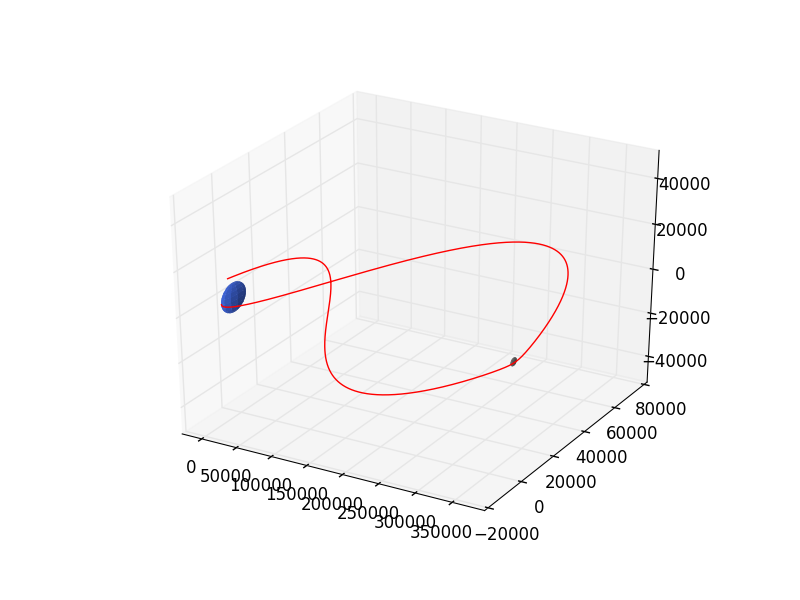
\includegraphics[width=20em]{chaos_app01_01.png}

Kaynaklar

[1] Stack Exchange, {\em Restricted Three-Body Problem}, \url{http://math.stackexchange.com/questions/54735/restricted-three-body-problem}


\end{document}

